\documentclass[a4paper,11pt]{article}
\pdfoutput=1 % if your are submitting a pdflatex (i.e. if you have
             % images in pdf, png or jpg format)

\usepackage{jheppub} % for details on the use of the package, please
                     % see the JHEP-author-manual

\usepackage[T1]{fontenc} % if needed
\usepackage{tikz}
\usepackage{tikz-network}
\usepackage{xcolor}
\usetikzlibrary{patterns}
\usetikzlibrary{matrix,positioning,fit}
\usetikzlibrary{calc}
\newdimen\R
\R=1.5cm

\usepackage{dcolumn}
\newcolumntype{L}{D{.}{.}{2,8}}

\newcommand{\beq}{\begin{equation}}
\newcommand{\eeq}{\end{equation}}


\title{\boldmath  On the crossing symmetry properties of twist fields correlation functions associated to genus 2 Riemann surfaces}


%% %simple case: 2 authors, same institution
%% \author{A. Uthor}
%% \author{and A. Nother Author}
%% \affiliation{Institution,\\Address, Country}

% more complex case: 4 authors, 3 institutions, 2 footnotes
\author[a]{Filiberto Ares,\note{Corresponding author.}}
\author[b]{R. Santachiara,}
\author[c, d]{J. Viti}

% The "\note" macro will give a warning: "Ignoring empty anchor..."
% you can safely ignore it.

\affiliation[a]{International Institute of Physics, UFRN, \\ Campos Universit\'ario, Lagoa Nova 59078-970 Natal, Brazil}
\affiliation[b]{Universit\'e Paris-Saclay,  CNRS,  LPTMS,  \\ 91405,  Orsay,  France}
\affiliation[c]{International Institute of Physics \& ECT, UFRN, \\ Campos Universit\'ario, Lagoa Nova 59078-970 Natal, Brazil}
\affiliation[d]{INFN, Sezione di Firenze, \\ Via G. Sansone 1, 50019 Sesto Fiorentino, Firenze, Italy}
% e-mail addresses: one for each author, in the same order as the authors
\emailAdd{first@one.univ}
\emailAdd{second@asas.edu}
\emailAdd{third@one.univ}
\emailAdd{fourth@one.univ}




\abstract{We calculate the CFT partition function on genus two Riemann surface by
using the conformal bootstrap.}



\begin{document} 
\maketitle
\flushbottom

\section{Introduction}
\label{sec:intro}

\section{CFT partition functions on Renyi surfaces}
Let us consider a conformal field theory $\mathcal{C}$, with central charge 
$c$, living on a Riemann surface $\Sigma_g$ of genus $g$. In the following we will refer to $\mathcal{C}$ as the seed theory. 
Let us consider the family of Renyi Riemann surfaces $\Sigma_g(x)$ of 
genus $g=N-1$ described by the  complex algebraic curve
\begin{equation}\label{riemann_surf}
\Sigma_{N-1}(x): \quad  w^N=\frac{z(z-1)}{z-x},
\end{equation}
which has branch points of order $N$ at $z_{\text{branch}}=0$, $x$, $1$, and $\infty$. The Eq.~\eqref{riemann_surf} can be interpreted as an $N$-sheet cover of the Riemann sphere $\mathbb C\cup \{\infty\}$ parametrized by $z$. For a visualization of the surface on $\mathbb C^2$ we refer to~\cite{Dubrovin}. These Riemann surfaces are parametrized by  
the complex number $x$ and enjoy a symmetry $\mathbb{Z}_N$ since 
Eq.~\eqref{riemann_surf} is invariant under the transformation 
$w\mapsto e^{\frac{2\pi i k}{N}}w$, with $k\in\mathbb{N}$. 
This transformation amounts to a cyclic permutation of the $N$ sheets of the surface, where each sheet is labelled by the choice of the branch of the $N$-root in Eq.~\eqref{riemann_surf}. 

\noindent In the following we consider the following quantity:
\begin{equation}
\mathcal{Z}_{N-1}(x)=\text{Partition function of $\mathcal{C}$ on the surface  $\Sigma_{N-1}(x)$, defined in \ref{riemann_surf}}.
 \end{equation}
The CFT partition function on $\Sigma_{N-1}(x)$ is strictly related to the orbiforld CFT $\mathcal{C}^{\otimes N}/Z_N$ that lives on the Riemann sphere $z$ \cite{Dixon, Knizhnik}. In this respect a crucial role is played by the $\mathbb Z_N$ twist and anti-twist field $\sigma_N$ and $\bar{\sigma}_N$, that are  spinless primary fields of conformal dimension~\cite{Knizhnik}
\begin{equation}
 h_{\sigma_N}=\bar{h}_{\sigma_N}=\frac{c}{24}\left(N-\frac{1}{N}\right);
\end{equation}
\noindent More specifically, the partition function $\mathcal{Z}_{N-1}(x)$ is given by the four-point function of twist fields inserted at the branch points $z=z_{branch}=\{0,1,x,\infty\}$: 
\begin{equation}
\label{geom_inter}
\mathcal{Z}_{N-1}(x)=\langle \sigma_N (\infty) \bar{\sigma}_N(1)\sigma_N(x,\bar{x}) \bar{\sigma}_N(0)\rangle,
 \end{equation}

%Given for instance a  $\mathcal C^{\otimes N}$ primary $\boldsymbol{O}^{(k)}(z)=\mathbb I^{(1)}\otimes\mathbb I\dots\otimes O^{(k)}(z)\otimes\dots\otimes\mathbb I^{(N)}$, the multivaluedness of its correlation functions under the analytic continuation $(z-z_{\text{branch}})\mapsto e^{2\pi i}(z-z_{\text{branch}})$ is implemented by the twist field inserted at the branch point:
%\begin{equation}
%\label{nonloc}
% \boldsymbol {O}^{(k)}(e^{2\pi i}(z-z_{\text{branch}}))\sigma_N(z_{\text{branch}})\mapsto \boldsymbol{O}^{(k+1)}(z-z_{\text{branch}})\sigma_N(z_{\text{branch}}).
%\end{equation}
%Analogously, the anti-twist field $\bar{\sigma}_N(a)$, with the same conformal dimensions as $\sigma_N$, implements an anticyclic permutation:
% \begin{equation}
%\label{anonloc}
% \boldsymbol {O}^{(k)}(e^{2\pi i}(z-z_{\text{branch}}))\bar{\sigma}_N(z_{\text{branch}})\mapsto \boldsymbol{O}^{(k-1)}(z-z_{\text{branch}})\bar{\sigma}_N(z_{\text{branch}}).
%\end{equation}

\noindent Note that, due to the tranformation Eq.(\ref{riemann_surf}), the metric in $\Sigma_{N-1}(x)$ is non trivial.  Via a Weyl transformation, the corresponding partition function $\mathcal{Z}_{N-1}$ can then be put in relation to the partition function $\mathcal{\hat{Z}}_{N-1}$ on a Riemann surfaces with a flat metric\cite{Lunin}:  
\begin{equation}\label{partition_twist_correl}
 \mathcal{\hat{Z}}_{N-1}(x)=e^{cS_{\text{anom.}}(x)} \mathcal{Z}_{N-1}(x),
\end{equation}
where the prefactor $e^{cS_{\text{anom.}}(x)}$ in Eq.~\eqref{partition_twist_correl} is the Weyl anomaly originating from the metric transformation.
%It takes into account that in the orbifold approach the metric employed to determine the partition function on $\Sigma_{N-1}(x)$ is a flat metric on each sheet of the surface with conical singularities at the branch points of the covering map. The partition function with a flat metric $\mathcal{Z}_{N-1}$ is then related to the latter by  the prefactor in Eq.~\eqref{partition_twist_correl} which can be explicitely calculated.  
\noindent The Weyl anomaly can be explictely calculated. Take for instance the case $N=2$, where, under the Abel-Jacobi map, $\Sigma_{1}(x)$ is conformally equivalent to a flat torus of modulus 
\begin{equation}\label{tau}
 \tau(x)=i\frac{K(1-x)}{K(x)}, 
\end{equation}
where $K(x)$ is the complete elliptic integral of first 
kind~\cite{Whittaker}. Correspondingly, the CFT partition function $\mathcal{\hat{Z}}_1(x)$ on a flat torus 
with modulus $\tau(x)$ is~\cite{Lunin}
\begin{equation}\label{partition_torus_twist}
 \mathcal{\hat{Z}}_1(x)=|2^8 x(1-x)|^{c/12} \mathcal{Z}_{N-1}(x)=|2^8 x(1-x)|^{c/12} \langle \sigma_2 (\infty)\bar{\sigma}_2(1)\sigma_2(x, \bar{x})\bar{\sigma}_2(0)\rangle.
\end{equation}
Finally, $\mathcal{Z}_{N-1}$ must be invariant  
under modular transformations~\cite{CardyMod, Cappelli, Cappelli2}.  For the class of surfaces $\Sigma_{N-1}(x)$, the moduli space is one-dimensional and modular invariance implies the crossing
symmetry of the twist field four-point correlation function~\cite{Cardy},
\begin{equation}\label{cross_symmetry}
 \langle \sigma_N(\infty)\bar{\sigma}_N(1)\sigma_N(1-x, 1-\bar{x})\bar{\sigma}_N(0)\rangle=
 \langle \sigma_N(\infty)\bar{\sigma}_N(1)\sigma_N(x, \bar{x})\bar{\sigma}_N(0)\rangle. 
\end{equation}
For example, if we consider a torus with modulus $\tau$ that of Eq.~\eqref{tau},
then the modular transformation $\tau\mapsto-1/\tau$ induces the change
$x\mapsto 1-x$. An analogous observation holds for $\Sigma_{2}(x)$, as discussed in~\cite{Cardy}.
 We will focus in particular on 
the symmetry $x\mapsto 1-x$ of the twist field correlation function for $N=3$. 
%The idea of using the crossing simmetry of the twist field correlation function to calculate higher genus CFT partition function was firstly  proposed in~\cite{ZamolodchikovAT}.


\section{Modular conformal blocks}\label{sec:conf_blocks}
The twist fields four-point 
function of the orbifold theory admits the following expansion:
\begin{equation}\label{conformal_block_decomposition_0}
 \langle \sigma_N (\infty)  \bar{\sigma}_N(1) \sigma_N (z, \bar{z})\bar{\sigma}_N(0)\rangle=
 \sum_{\boldsymbol{h},\boldsymbol{\bar{h}}} D_{\boldsymbol{h}, \boldsymbol{\bar{h}}}
 \mathcal{G}_{c, \boldsymbol{h}}^{(N)}(z)\mathcal{G}_{c,\boldsymbol{\bar{h}}}^{(N)}(\bar{z}),
\end{equation}
where $\boldsymbol{h}\equiv\{h_1, \dots, h_N\}$ with $h_j$ being the conformal dimension of  
a primary in the seed theory.
The function $\mathcal{G}_{c, \boldsymbol{h}}^{(N)}(z)$, defined below, are the so-called modular conformal blocks.  They are normalized such that: 
\begin{equation}
\mathcal{G}_{c, \boldsymbol{h}}^{(N)}(z)=z^{\;|\boldsymbol{h}| -2\; h_{\sigma_N}}\left(1+ O(z)\right),
\end{equation}
where $|\boldsymbol{h}|=\sum_j h_j$ and are fixed by the orbifold symmetry algebra. The $\mathcal{G}_{c, \boldsymbol{h}}^{(N)}(z)$ encode therefore the universal part of the orbifold correlation function  while  the structure constants  $D_{\boldsymbol{h}, \boldsymbol{\bar{h}}}$  characterize the specific bootstrap solution under consideration. Note that in Eq.\eqref{conformal_block_decomposition_0}, we inserted one twist field at a general point $(z,\bar{z})$ on the Riemann sphere to stress the fact we are computing a standard CFT correlation function on the $z$-sphere. To recover the geometric interpretations of Eqs.~\eqref{riemann_surf} -\eqref{geom_inter}, one sets $z,\bar{z}\to x,\bar{x}$.

\noindent We review the procedure, well described in \cite{Collier}, to obtain the small $z$ expansion  of  the modular conformal blocks.  Let us fix some notations. In the seed CFT $\mathcal{C}$, we denote by $\phi_{h}(z)$  an holomorphic primary fields of dimension $h$  and by $X_{h}^{M}(z)$ one of its descendants. We label with  $M\equiv\{m_1,\dots,m_q\}$ a partition of the integer  $|M|$.  In terms of the  Virasoro generators $L_{-m}(z)$, defined in Eq.~\eqref{vir_ln}, $\phi_{h}^{M}(z)$ takes the form:
\begin{equation}
\label{desc}
 \phi_{h}^{M}(z):=L_{-M}(z)\;\phi_h(z)~~{\rm{where}}~~ L_{-M}(z):=L_{-m_1}(z)\dots L_{-m_q}(z).
 \end{equation}
The field  $X_{h}^{M}(z)$ has conformal dimension $h+|M|$. Using the field-state correspondance $|\phi_{h}\rangle\equiv \lim_{z\to 0}\phi(z)|0\rangle$, with $|0\rangle$ the vacumm in $\mathcal{C}$ and the Virasoro scalar product \cite{DiFrancesco}, we denote by  $G^{h}_{M_1,M_2}$ the Virasoro Kac-Shapovalov matrix:
\begin{equation}
G^{h}_{M_1,M_2} = \langle \phi_{h}^{M_1}|\phi_{h}^{M_2}\rangle. 
\end{equation}
The scalar product can be written in terms of correlation function by using the correspondence  $\langle \phi_{h} |\equiv\lim_{z\rightarrow\infty}z^{2h}\langle 0|\phi(z)$ where $\langle 0|$ is the dual of the vaccuum state. If not explicitily stated otherwise, in what follows we consider irriducible Virasoro representation, i.e. without descendant states with vanishing norm, refered here as null-vectors. The role of null-vectors will be considered more in detail in Sec. (\ref{null_vec1}).  

\noindent In the replicated theory  $\mathcal{C}^{\otimes N}$, an holomorphic primary $\boldsymbol{\phi}_{\boldsymbol{h}}(z)$  is labelled by the vector of dimension $\boldsymbol{h}$ and it has conformal dimension $|\boldsymbol{h}|$. The primary in the replicated theory $\boldsymbol{\phi}_{\boldsymbol{h}}(z)$ is expressed in terms of the seed theory primaries as:
\begin{equation}
\boldsymbol{\phi}_{\boldsymbol{h}}(z)=\phi_{h_1}(z)\otimes \cdots\otimes \phi_{h_N}(z).
\end{equation}
Using the symbol $\boldsymbol{M}$ to indicate a vector of $N$ partitions of  $|M_1|,\dots, |M_N|$, $\boldsymbol{M}\equiv\{M_1,\dots,M_N\}$,  the  $\mathcal{C}^{\otimes N}$ descendants are denoted by  $\boldsymbol{\phi}^{\boldsymbol{M}}_{\boldsymbol{h}}(z)$
 \begin{equation}
 \boldsymbol{\phi}_{\boldsymbol{h}}^{\boldsymbol{M}}(z)=\phi_{h_1}^{M_1}(z)\otimes \dots \otimes \phi_{h_N}^{M_N}(z).
\end{equation}
They have conformal dimension $|\boldsymbol{h}|+|\boldsymbol{M}|$, where $|\boldsymbol{M}|=\sum_j |M_j|$. 
The corresponding scalar product matrix $\boldsymbol{G}^{\boldsymbol{h}}_{\boldsymbol{M}_1\boldsymbol{M}_2}$, of size $\prod_{j=1}^{N}|M_j|^2\times \prod_{j=1}^{N}|M_j|^2$, takes the following form:
\begin{equation}
\label{scal}
 \boldsymbol{G}^{\boldsymbol{h}}_{\boldsymbol{M}_1\boldsymbol{M}_2}:=\langle \boldsymbol{\phi}_{\boldsymbol{h}}^{\boldsymbol{M}_1} | \boldsymbol{\phi}_{\boldsymbol{h}}^{\boldsymbol{M}_2}\rangle=\prod_{j=1}^N G^{h_j}_{M_j,M_j'}.
\end{equation}
We will also use $\boldsymbol{0}$ to indicate the empty partition $\boldsymbol{M}=\{\{0\},\cdots,\{0\}\}$. In these notations, $\boldsymbol{\phi}_{\boldsymbol{h}}=\boldsymbol{\phi}_{\boldsymbol{h}}^{\boldsymbol{0}}$. Moreover the local descendant fields, entering in the correlation functions, are obtained by gluing the holomorphic and anti-holomorphic part:
\begin{equation}
\boldsymbol{\phi}^{\boldsymbol{M},\boldsymbol{\bar{M}}}_{\boldsymbol{h},\boldsymbol{\bar{h}}} (z,\bar{z})=\boldsymbol{\phi}^{\boldsymbol{M}}_{\boldsymbol{h}}(z)\boldsymbol{\phi}^{\boldsymbol{\bar{M}}}_{\boldsymbol{\bar{h}}}(\bar{z}), \quad 
\end{equation} 

\noindent As well known in the theory of conformal blocks \cite{DiFrancesco}, the small $z$ representation of $\mathcal{G}_{c, \boldsymbol{h}}^{(N)}(z)$ can be obtained obtained by inserting an identity resolution
in the representation $\boldsymbol{h}$. One obtains the following expression: 
\begin{equation}\label{conformal_block_decomposition}
 \mathcal{G}_{c,\boldsymbol{h}}^{(N)}(z)=
 z^{|\boldsymbol{h}|-2h_{\sigma_N}}\sum_{\substack{\boldsymbol{M}_1, \boldsymbol{M}_2 \\ |\boldsymbol{M}_1|=|\boldsymbol{M}_2|} } z^{|\boldsymbol{M}_1|}\;\Gamma^{*}_{\boldsymbol{h}, \boldsymbol{M}_1}\; [\boldsymbol{G}^{\boldsymbol{h}}_{\boldsymbol{M}_1,\boldsymbol{M}_2}]^{-1}\;\Gamma_{\boldsymbol{h},\boldsymbol{M}_2}
\end{equation}
where the $\Gamma_{\boldsymbol{h},\boldsymbol{M}}$ and $\Gamma^{*}_{\boldsymbol{h},\boldsymbol{M}}$ are matrix element between descendant fields.  In terms of the orbifold structure constant:
\begin{equation}
C_{\boldsymbol{h},\boldsymbol{\bar{h}}}=\langle  \sigma_{N}|\bar{\sigma}_{N}(1)|\boldsymbol{\phi}_{\boldsymbol{h},\boldsymbol{\bar{h}}}\rangle,
\end{equation}
one has: 
 \begin{equation}
\Gamma_{\boldsymbol{h},\boldsymbol{M}} = \frac{\langle \boldsymbol{\phi}^{\boldsymbol{M},\boldsymbol{0}}_{\boldsymbol{h},\boldsymbol{\bar{h}}}| \sigma_{N}(1)|\bar{\sigma}_{N}\rangle}{C_{\boldsymbol{h},\boldsymbol{\bar{h}}}},\quad  \Gamma^{*}_{\boldsymbol{h},\boldsymbol{M}} = \frac{\langle  \sigma_{N}|\bar{\sigma}_{N}(1)|\boldsymbol{\phi}^{\boldsymbol{M},\boldsymbol{0}}_{\boldsymbol{h},\boldsymbol{\bar{h}}}\rangle}{C_{\boldsymbol{h},\boldsymbol{\bar{h}}}} .
 \end{equation}
 The matrix elements  $\Gamma_{\boldsymbol{h},\boldsymbol{M}}$ and $\Gamma^{*}_{\boldsymbol{h},\boldsymbol{M}}$ have an algebraic nature, in the sense that they are fixed by the orbifold algebra. The structur constants, on the other hand, can depend on the model under consideration. Comparing with the expansion Eq.\eqref{conformal_block_decomposition_0}, one has:
 \begin{equation}
 D_{\boldsymbol{h},\boldsymbol{\bar{h}}}= \left(C^{\boldsymbol{h},\boldsymbol{\bar{h}}}\right)^2
 \end{equation}
\subsection{Computing the three point functions by unfolding}
The computation of the orbifold correlation function reduces then to the one of the three-point function
\begin{equation}\label{orbifold_three-point}
 \Gamma_{\boldsymbol{h},\boldsymbol{M}} \;C_{\boldsymbol{h},\boldsymbol{h}} = \langle \boldsymbol{\phi}^{\boldsymbol{M},\boldsymbol{0}}_{\boldsymbol{h}}(\infty) \sigma_{N}(1)\bar{\sigma}_{N}(0)\rangle.
\end{equation}
In this respect, it is very useful, especially for $N=2$ and $N=3$,  to consider a $N$-to-one conformal map
$t\mapsto z(t)$ with branch points at $z_{\text{branch}}=\{0, 1\}$  that behaves as $z-z_{\text{branch}}\sim (t-t_{\text{branch}})^N$~\cite{Lunin}.
That is, the $t$-surface is a $N$-sheet cover with genus zero 
 of the $z$-Riemann sphere with a branch cut along 
$(0,1)$. We will refer to the $t-$ surface as the $t$-Riemann sphere. Without losing in generality, let's consider the holomorphic part of the correlation function. The point $z=\infty$, where the field $\boldsymbol{\phi}^{\boldsymbol{M}}_{\boldsymbol{h}}$  is inserted, is mapped to $N$ different points $t_\infty=\{t_1, \dots, t_N\}$ in 
the covering space. Let us denote by $\tilde{\phi}_{h_j}^{M_j}(t_j)$ the image
of the field $\phi_{h_j}^{M_j}(\infty)$ under the covering map $t\mapsto z(t)$:
\begin{equation}
\label{Jac}
\tilde{\phi}_{h_j}^{M_j}(t_j) = \left(\left.\frac{d z(t)}{d t}\right|_{t=t_j} \right)^{-h_j} \mathcal{L}_{-M_j}(t_j)\;\phi_{h_j} (z(t_j)),
\end{equation}
where the $\mathcal{L}_{-M_j}(t_j)$ are the transformed Virasoro generators living on the $t$- surface. Once the $\mathcal{L}_{-M}(\infty)$and  $\mathcal{L}_{-M}(0)$ are expressed in terms of the $L_{n}$ generators on the $z$ Riemann sphere, see Appendix. 
The role of this map is therefore to unfold the field of the replicated theory living on the $z$- Riemann surface:
\begin{equation}
\{\tilde{\phi}_{h_j}^{M_j}(t_j)\}_{j=1,\cdots,N}\mapsto \boldsymbol{\phi}_{\boldsymbol{h}}^{\boldsymbol{M}}(\infty),
\end{equation}

 The  orbifold  three-point function (\ref{orbifold_three-point})  is then transformed into the $N$-point function on $t$-sphere:
\begin{equation}\label{N-point}
\langle \boldsymbol{\phi}^{\boldsymbol{M}}_{\boldsymbol{h}}(\infty) \sigma_{N}(1)\bar{\sigma}_{N}(0)\rangle=\langle \tilde{\phi}^{M_1}_{h_1}(t_1)\cdots\tilde{\phi}_{h_N}^{M_N}(t_N)\rangle.
\end{equation}


 

\subsection{Explicit calculations of modular conformal blocks: the case $N=2$}
Let us illustrate the unfolding method first in the case $N=2$. Here  we can use the unfolding  map
\begin{equation}\label{g_one_covering_map}
 z(t)=\frac{(t+1)^2}{4t},
\end{equation}
under which  $t_{\infty}=\{0,\infty\}\mapsto z=\infty$.
Using Eq.~\eqref{Jac}, the  Eq.~\eqref{N-point}  becomes:
\begin{equation}\label{C_2_X}
 \langle \boldsymbol{\phi}^{\{M_1,M_2\}}_{\{h_1,h_2\}}(\infty) \sigma_{N}(1)\bar{\sigma}_{N}(0)\rangle=\langle \tilde{\phi}_{h_1}^{M_1} | \tilde{\phi}_{h_2}^{M_2}\rangle=
 \delta_{h_1, h_2}\delta_{|M_1|,|M_2|}\;2^{-4 h_1} \;\rho^h_{M_1,M_2},
\end{equation}
where $\rho$ is the symmetric $|M_1|\times|M_1|$ matrix
\begin{equation}
\label{rho}
 \rho^h_{M_1,M_2}:=\langle \mathcal{L}_{-M_1}\phi_{h}|\mathcal{L}_{-M_2}\phi_{h}\rangle.
\end{equation}
In the above expression,  the $\mathcal{L}$ are meant to be expressed in terms of the $L$  ones, see Eqs.~\eqref{g1_1} and~\eqref{g1_2},/ The matrix $\rho^h$  can be easily computed using the standard Ward identities, see Eq.~\eqref{wardvir1} and Eq.~\eqref{wardvir2}. 
Using Eq.\eqref{C_2_X} in Eq.\eqref{conformal_block_decomposition}, one arrives at the expression
\begin{equation}\label{genus_one_conf_block}
 \mathcal{G}_{c, h}^{(2)}(z)=\sum_{M_1, M_2}\sum_{N_1, N_2}
 z^{2h-c/8+|M_1|+|M_2|}[G^{h}_{M_1,N_1}]^{-1}[G^{h}_{ M_2,N_2}]^{-1}
 \rho^h_{M_2,M_1}\rho^h_{N_2,N_1}.
\end{equation}
By recalling that the matrices $G^h$ and $\rho^h$ are symmetric, the coefficients of the combinatorial 
expansion in Eq.~\eqref{genus_one_conf_block} can be organized as 
matrix products, presented in the diagram of Fig.~\ref{fig-g1}. 

\noindent Let recall that the torus partiction $\mathcal{\hat{Z}}_1(x)$ is a sesquilinear form of irreducible Virasoro characters $\chi_{h}(\tau(x))$~\cite{Cappelli, Cappelli2}:
\begin{equation}
\mathcal{\hat{Z}}_1(x) = \sum_{h,\bar{h}} \chi_{h}(\tau(x)) \chi_{\bar{h}}(\bar{\tau}(x)),
\end{equation}
where 
\begin{equation}
\chi_{h}(\tau(x)) = e^{2\pi i \tau(x)\left(h-\frac{c}{24}\right)}\left(1+ o\left(e^{2\pi i \tau(x)}\right)\right) \sim \left(\frac{x}{16}\right)^{ 2 h-\frac{c}{12}}, \quad \text{for}\; x<<1
\end{equation}
 By comparing this expression  to Eqs.~\eqref{partition_torus_twist}  and (\ref{conformal_block_decomposition_0}), one indeed identifies 
\begin{equation}\label{character_conf_block}
\mathcal{G}_{c,h}^{(2)}(x)=2^{-c/3}[x(1-x)]^{-c/24}\chi_{h}(\tau(x)),\quad  D_{\{ h_1, h_2 \}, \{ \bar{h}_1,\bar{h}_2\} } =\delta_{h_1,h_2}\;\delta_{\bar{h}_1,\bar{h}_2} \;2^{-8 (h_1+\bar{h}_1)}
\end{equation}



\begin{figure}[t]
\centering
 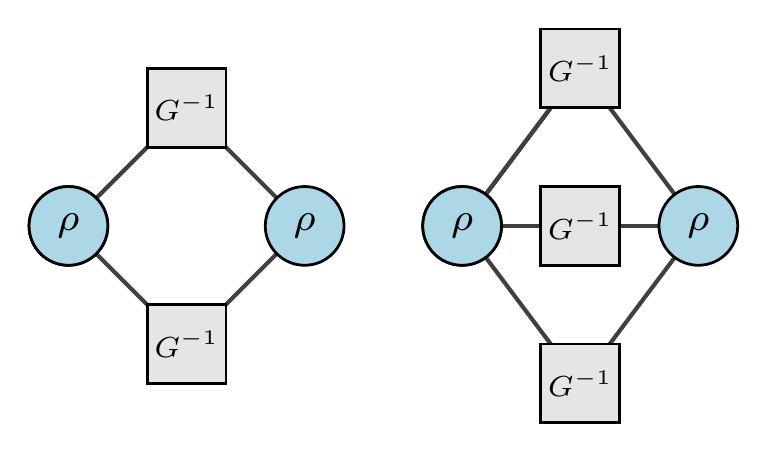
\begin{tikzpicture}
  \Vertex[size=1, label=$\rho$, fontscale=2]{A};
  \Vertex[x=1.5, y=1.5, size=1, shape=rectangle, color=gray!20, label=$G^{-1}$, fontscale=1.5]{B};
  \Vertex[size=1, label=$\rho$, fontscale=2]{A};
  \Vertex[x=3, y=0, size=1, label=$\rho$, fontscale=2]{C};
  \Vertex[x=1.5, y=-1.5, size=1, shape=rectangle, color=gray!20, label=$G^{-1}$, fontscale=1.5]{D};
  \Edge(A)(B);
   \Edge(B)(C);
    \Edge(C)(D);
     \Edge(D)(A);
     \begin{scope}[xshift= 5cm]
      \Vertex[size=1, label=$\rho$, fontscale=2]{A};
  \Vertex[x=1.5, y=2, size=1, shape=rectangle, color=gray!20, label=$G^{-1}$, fontscale=1.5]{B};
  \Vertex[size=1, label=$\rho$, fontscale=2]{A};
  \Vertex[x=3, y=0, size=1, label=$\rho$, fontscale=2]{C};
  \Vertex[x=1.5, y=-2, size=1, shape=rectangle, color=gray!20, label=$G^{-1}$, fontscale=1.5]{D};
  \Vertex[x=1.5, y=0, size=1, shape=rectangle, color=gray!20, label=$G^{-1}$, fontscale=1.5]{E};
  \Edge(A)(B);
  \Edge(A)(B);
   \Edge(B)(C);
    \Edge(C)(D);
     \Edge(D)(A);
     \Edge (A)(E);
     \Edge (E)(C);
     \end{scope}

 \end{tikzpicture}
\caption{On the left: Matrix product representation of the genus one conformal block in Eq.~\eqref{genus_one_conf_block}. On the right: Matrix product representation of the genus two conformal block in Eq.~\eqref{genus_two_conf_block}.}
\label{fig-g1}
\end{figure}
\subsection{Explicit calculations of modular conformal blocks: the case $N=2$}

For $N=3$, the orbifold three-point correlation 
function of Eq.~\eqref{orbifold_three-point} can be computed 
by considering the three-to-one map~\cite{Collier}
\begin{equation}\label{g_two_covering_map}
 t\mapsto z =\frac{(t+\omega)^3}{3\omega(1-\omega)t(t-1)},\quad \omega=e^{\frac{2\pi i}{3}}.
\end{equation}
This transformation has branch points of order three at 
$z=0$ and $1$ and maps $z=\infty$  to the set of points 
$t_{\infty}=\{0, 1, \infty\}$ in the $t$-space.
The images $\mathcal{L}_{-n}(t_{\infty})$ of the Virasoro descendent $L_{-n}(z=\infty)$ 
under Eq.~\eqref{g_two_covering_map} can be obtained, as in the 
case of genus one, by using Eq.~\eqref{Virasoro_transf}.
Then we have, for $n\geq 1$,
\begin{equation}
 \mathcal{L}_{-n}(t_{\infty})=\sum_{m\geq -n} a_{nm}^{t_{\infty}}L_m(t=t_\infty)+\frac{c}{27}(n-1),
\end{equation}
where the coefficients $a_{nm}^{t_{\infty}}$ can be determined in closed form from the residue theorem, see also Eq.~(2.9)
of Ref.~\cite{Collier}. The $\mathbb{C}$-number $C_3^{\boldsymbol{h},\boldsymbol{M}}$ in Eq.~\eqref{conformal_block_decomposition} is the three-point function on the $t$-sphere:
\begin{equation}\label{C_3_X}
 C_3^{\boldsymbol{h},\boldsymbol{M}}=\langle \mathcal{X}_{h_1}|\mathcal{X}_{h_2}(1)|\mathcal{X}_{h_3} 
 =[3\omega(1-\omega)]^{-h_1-h_2-h_3}C_{h_1h_2h_3}\rho_{M1,M2,M3}^{h_1,h_2,h_3}
\end{equation}
where $C_{h_1 h_2 h_3}=\langle \phi_{h_1}|\phi_{h_2}(1)|\phi_{h_3}\rangle$ is a structure constant in the seed CFT, while the symmetric tensor $\rho^{h_1,h_2,h_3}$ is 
\begin{equation}
 \rho^{h_1,h_2,h_3}_{M_1,M_2,M_3}:=
 \frac{\langle \boldsymbol{\mathcal{L}}_{-M_1}\phi_{h_1}|\boldsymbol{\mathcal{L}}_{-M_2}(1)\phi_{h_2}(1)|\boldsymbol{\mathcal{L}}_{-M_3}\phi_{h_3}\rangle}
 { \langle \phi_{h_1}|\phi_{h_2}(1)|\phi_{h_3}\rangle}.
\end{equation}

From Eq.~\eqref{C_3_X}, it follows that the number of genus two conformal block is in one-to-one correspondence~\cite{Cardy, Collier} with the number of non-zero structure constants of $\mathcal{C}$.
From Eq.~\eqref{conformal_block_decomposition}, we can eventually deduce the following matrix-product representation
for the genus two conformal block \cite{Collier}
\begin{equation}\label{genus_two_conf_block}
 \mathcal{G}_{c, h_1, h_2, h_3}^{(3)}(z)=
 2^{-4\sum\limits_{j=1}^3h_j}
 \sum_{\{M_j\}}\sum_{\{N_j\}}
 z^{-2c/9+\sum\limits_{j=1}^3(h_j+|M_j|)}
 \prod_{j=1}^3 [G_{M_j,N_j}^{h_j}]^{-1}
 \rho^{h_1,h_2,h_3}_{M_1,M_2,M_3}[\rho_{N_1,N_2,N_3}^{h_1,h_2,h_3}]^*,
\end{equation}
which is also illustrated in Fig.~\ref{fig-g1}.
The conformal block $\mathcal{G}_{c, h_1, h_2, h_3}^{(3)}$ in Eq.~\eqref{genus_two_conf_block} is
manifestly symmetric under permutations of $h_1$, $h_2$ and $h_3$, consistently with the $\mathbb Z_3$ (in fact $S_3$) symmetry of the untwisted orbifold sector.

\subsection{Handling null vectors}
\label{null_vec1}
We discuss now the case of where the seed theory is a Virasoro minimal model. These theories are built by removing zero-norm states and their descendents from the Verma modules of the Virasoro algebra.  As a consequence, they contain only a finite number of primary fields and are known as minimal models~\cite{BPZ}. 
As it is well known, some of the Virasoro Verma modules with $c<1$  have 
null vectors  that must be eliminated to construct irreducible (also called degenerate~\cite{Ribault}) representations of the minimal model conformal algebra.
Contributions of spurious null vectors 
are nevertheless present in the expansion of Eq.~\eqref{genus_one_conf_block}, since the latter includes \textit{a priori} all the states within a Verma module. Therefore, a correct definition of higher genus conformal blocks for a rational seed CFTs  must be supplemented with a regularization scheme that removes them. A simple procedure is outlined in the following. 



Let us assume that the Virasoro representation labelled by $(c, h)$
contains a null vector, and suppose to choose a basis  that   includes it. The null vector and its descendent are orthogonal to all 
vectors of the basis, thus the representation is reducible.  Observe now, see also Fig.~\ref{fig-g1}, that the inverse of the Gram matrix appears twice in the
genus one conformal block of Eq.~\eqref{genus_one_conf_block}. The 
entries of the inverse Gram matrix are proportional to $[\det(G^h)]^{-1}$ 
and, therefore, are singular when the null vector is among the basis 
elements. As already emphasized, the scalar products $\rho^h$ in Eq.~\eqref{genus_one_conf_block} 
vanish instead. In order to eliminate the null vector contribution from Eq.~\eqref{genus_one_conf_block} is then
enough, if $h\neq0$, to modify the central charge dependence of both 
$\rho^h$ and $G^h$ as follows 
\begin{equation}\label{regularization}
 \rho^h|_{c+\varepsilon^2}, G^h|_{c+\varepsilon},
\end{equation}
with $\varepsilon>0$. In this way, in the limit $\varepsilon\to 0$, the matrix elements of $\rho^h$ between a null vector and any other basis state is $O(\varepsilon^2)$ while the determinant of $G^h$ is $O(\varepsilon)$. Therefore null vectors contributions are at most $O(\varepsilon^2)$ and drop in the $\varepsilon\rightarrow 0$ limit, see also~\cite{SV, Javerzat, Alkalaev}.

We denote by $\tilde{\mathcal{G}}_{c, h}^{(2)}(z)$ the regularized conformal 
block obtained by the prescription in Eq.~\eqref{regularization} in the limit $\varepsilon\to 0$. 
For instance  for $c=1/2$ and $h=1/16$, the first few terms in the regularized expansion of Eq.~\eqref{genus_one_conf_block} about $z=0$ are
\begin{equation}
 \tilde{\mathcal{G}}_{\frac{1}{2},\frac{1}{16}}^{(2)}(z)=
 \frac{z^{1/8}}{\sqrt{2}}\left[1+\frac{z}{16}+\frac{17 z^2}{512}
 +\frac{187 z^3}{8192}+\frac{9163 z^4}{524288}+O(z^5)\right].
\end{equation}
The coefficient of the $O(z^4)$ term will be different if the regularization
scheme is not implemented. Indeed the Verma module $(c=1/2,h=1/16)$ has a null vector at level two. If this vector was selected on both replicas of the seed theory, i.e. in the sector $|M_1|=|M_2|=2$ of Eq.~\eqref{genus_two_conf_block}, its contribution would be $O(1)$ in the expansion.
The power series of the regularized conformal block reproduces the expansion of the character $\chi_{c,h}(q)$ of the irreducible representation $(c,h)$. As usual, we defined $q(z)=e^{i\pi \tau(z)}$ with $\tau(z)$ given in Eq.~\eqref{tau}


It can be checked that the power series expansion about $z=0$ of the functions in Eq.~\eqref{character_conf_block} coincides order by order. For the case of the identity, $h=0$, we can follow a similar strategy but 
modifying in Eq.~\eqref{genus_one_conf_block} the dependence of the matrices $G^h$ and 
$\rho^h$ on $h$ instead of $c$ such as
\begin{equation}\label{regularization_identity}
 \rho^{h=\mu^2}, G^{h=\mu},
\end{equation}
with $\mu>0$. Then the limit $\mu\to 0$ produces the regularized 
conformal block $\tilde{\mathcal{G}}_{c, 0}^{(2)}(z)$ that
provides, using Eq.~\eqref{character_conf_block}, the  character of the irreducible representation of the identity.


In the case of minimal models with $c<1$, we also have to remove from the expansion in
Eq.~\eqref{genus_two_conf_block} the contribution of null vectors. We can eliminate it by
applying the same regularization prescription discussed in Eq.~\eqref{regularization}. In particular, the descendent three-point function $\rho^{h_1,h_2,h_3}$ will be $O(\varepsilon)$ when one of the states considered  has zero norm. This observation was already present in~\cite{Zamolodchikov2}.
Moreover, for $h_1=h_2=h_3=0$, we must apply the regularization 
scheme of Eq.~\eqref{regularization_identity}. Note that, according to Eq.~\eqref{C_3_X},
if the identity representation appears in only one of the copies, e.g. $h_1=0$, then 
we have to consider the same conformal family in the other two copies, i.e. $h_2=h_3$. In order 
to obtain the correct conformal block in this situation, one must take first $h_2=h_3$, with $h_1\neq0$,
and then perform the limit $h_1\to 0$.  As an example, let us consider the regularized 
genus two conformal block, which will be denoted by $\tilde{\mathcal{G}}_{c, h_1, h_2, h_3}^{(3)}(z)$,
for $c=1/2$, $h_1=h_2=1/16$ and $h_3=0$; the result is
\begin{equation}
 \tilde{\mathcal{G}}_{\frac{1}{2}, \frac{1}{16}, \frac{1}{16}, 0}^{(3)}(z)=
 \frac{z^{1/72}}{\sqrt{2}}\left[1 + \frac{7}{108}z + \frac{1595}{46656}z^2 + \frac{118405}{5038848}z^3 + 
 \frac{26160455}{1451188224}z^4 + O(z^5)\right].
\end{equation}
\section{Higher genus conformal blocks in terms of sphere conformal blocks}\label{app_sphere_conf_blocks}

In order to drastically improve the converge of the numerical bootstrap, it is necessary to expand the higher-genus conformal blocks $\mathcal{G}_{c,\boldsymbol{h}}^{(N)}(z)$ as a linear combination of sphere conformal blocks with central charge $Nc$. More specifically, we shall expect
\begin{equation}\label{expansion_sphere_conf_blocks}
 \mathcal{G}_{c, \boldsymbol{h}}^{(N)}(z)=\sum_{l=0}^{\infty}\alpha_{l}^{\boldsymbol{h}}
 \mathcal{F}_{Nc, |\boldsymbol{h}|+l}(z).
\end{equation}
In Eq.~\eqref{expansion_sphere_conf_blocks} above,  $\mathcal{F}_{Nc, |\boldsymbol{h}|+l}(z)$ is the sphere conformal block 
with central charge $Nc$, internal channel of conformal dimension $|\boldsymbol{h}|+l$, where $|\boldsymbol{h}|\equiv \sum_{j=1}^N h_j$, and external legs with fixed dimension 
$h_{\sigma_N}$. This function can be calculated
recursively by means of Zamolodchikov formula~\cite{Zamolodchikov2, Zamolodchikov}, see Appendix~\ref{app_zamolodchikov}.

In this Appendix, we discuss in more detail the expansion in Eq.~\eqref{expansion_sphere_conf_blocks} of the
conformal block $\mathcal{G}_{c, \boldsymbol{h}}^{(N)}(z)$ in terms of the conformal 
blocks on the sphere $\mathcal{F}_{Nc, |\boldsymbol{h}|+l}(z)$.

In each sheet of the orbifold theory $\mathcal{C}^{\otimes N}/\mathbb{Z}_N$, we 
can consider a copy $\boldsymbol{T}^{(j)}(z)$, $j=1,\dots, N$, of the stress-energy tensor of 
the seed theory $\mathcal{C}$. Then the stress-energy tensor of the 
orbifold theory $\boldsymbol{T}(z)$ is 
\begin{equation}\label{hatT}
 \boldsymbol{T}(z)=\sum_{j=1}^N \boldsymbol{T}^{(j)}(z).
\end{equation}
It generates transformations affecting all the sheets in the same way. 
Its Fourier modes,
\begin{equation}
 \boldsymbol{L}_n=\oint_{C_0}\frac{dz}{2\pi i} z^{n+1}\boldsymbol{T}(z),
\end{equation}
where $C_0$ is a contour encircling the point $z=0$, are symmetric 
under the exchange of sheets, 
\begin{equation}
 \boldsymbol{L}_n=\sum_{j=1}^N \boldsymbol{L}_n^{(j)}, \quad 
 \boldsymbol{L}_n^{(j)}=\mathbb{I}\otimes \overset{j}{\cdots} \otimes L_{n}\otimes \cdots \otimes \mathbb{I},
\end{equation}
and form a Virasoro algebra, 
\begin{equation}\label{symm_virasoro_alg}
 [\boldsymbol{L}_n, \boldsymbol{L}_{m}]=(n-m)\boldsymbol{L}_{n+m}+\frac{Nc}{12}n(n^2-1)\delta_{n+m, 0},
\end{equation}
with central charge $Nc$.

The conformal block $\mathcal{G}_{c, \boldsymbol{h}}^{(N)}(z)$ is associated with 
the field $\Phi_{\boldsymbol{h}}=\phi_{h_1}\otimes\cdots\otimes \phi_{h_N}$, where $\phi_{h_j}$ are 
primaries of $\mathcal{C}$ with chiral dimension $h_j$, and its descendents. 
Note that $\boldsymbol{L}_n\Phi_{\boldsymbol{h}}=0$ for all $n>0$ and $\boldsymbol{L}_0\Phi_{\boldsymbol{h}}=|\boldsymbol{h}| \Phi_{\boldsymbol{h}}$.
Then the contribution to $\mathcal{G}_{c, \boldsymbol{h}}^{(N)}(z)$ of the 
state $\Phi_{\boldsymbol{h}}$ and its \textit{symmetric} descendents $\boldsymbol{L}_{-M}\Phi_{\boldsymbol{h}}$ is given by 
the sphere conformal block $\mathcal{F}_{Nc, |\boldsymbol{h}|}(z)$, the first term
in the expansion of Eq.~\eqref{expansion_sphere_conf_blocks}. However, the states 
$\boldsymbol{L}_{-M}\Phi_{\boldsymbol{h}}$ do not span the full space of descendents of $\Phi_{\boldsymbol{h}}$ at each level. This is the reason why
other blocks appear in Eq.~\eqref{expansion_sphere_conf_blocks}. In fact, if we denote by $\mathfrak{p}(l)$
the number of partitions of the integer $l$, then there are $\mathfrak{p}(l)$ symmetric
descendents at level $l$. However, assumming that there are no null vectors, it is easy to check that 
at level $l$ the total number $\mathcal{N}_{N, l}$ of linear independent descendents of $\Phi_{\boldsymbol{h}}$ is
\begin{equation}
 \mathcal{N}_{N, l}=\sum_{\substack{Y, |Y|=l \\ |j_Y|\leq N}}\frac{N!}{(N-|j_Y|)!
 \prod_{i=1}^{|i_Y|}d_Y(i)!}\prod_{j=1}^{|j_Y|}\mathfrak{p}(i_Y(j)),
\end{equation}
where $Y$ denotes a partition of $l$. If we consider the Young tableau
associated to $Y$, then $|i_Y|$ and  $|j_Y|$ denote its number of columns and
rows respectively, $i_Y(j)$ is the number of columns in the row $j$ and 
$d_Y(i)$ is the number of rows with $i$ columns.


For example, let us consider the first level, $l=1$, of the orbifold theory 
with $N=3$. In this case, $\Phi_{\boldsymbol{h}}=\phi_{h_1}\otimes\phi_{h_2}\otimes\phi_{h_3}$ 
and we have a symmetric descendent $\boldsymbol{L}_{-1}\Phi_{\boldsymbol{h}}$. Since $\mathcal{N}_{3,1}=3$, 
we need two other states to form a basis for this level. Let us take them 
orthogonal to $\boldsymbol{L}_{-1}\Phi_{\boldsymbol{h}}$. The states orthogonal to it have the form
\begin{equation}
 \Psi(\lambda)=\left[\boldsymbol{L}_{-1}^{(1)}+\lambda \boldsymbol{L}_{-1}^{(2)}
 -\frac{h_1+\lambda h_2}{h_3} \boldsymbol{L}_{-1}^{(3)}\right]\Phi_{\boldsymbol{h}},
\end{equation}
where $\lambda$ is a complex parameter. One can check
that any vector in this orthogonal space is a primary, 
i.e. $\boldsymbol{L}_n \Psi(\lambda)=0$ for all $n>0$
and $\boldsymbol{L}_0\Psi(\lambda) = (h_1+h_2+h_3+1)\Psi(\lambda)$.
The contribution of these states and their symmetric descendents $\boldsymbol{L}_{-M}\Psi(\lambda)$
in the genus two conformal block $\mathcal{G}_{c, h_1, h_2, h_3}^{(3)}(z)$
is given by the sphere conformal block $\mathcal{F}_{3c, h_1+h_2+h_3+1}(z)$,
that is the second term in the expansion of Eq.~\eqref{expansion_sphere_conf_blocks}. In order to 
determine the corresponding structure constant $\alpha_{1}^{h_1, h_2, h_3}$, 
we choose and orthonormal basis $\{\Psi_1, \Psi_2\}$ of 
this orthogonal space. Then
\begin{eqnarray}
 \alpha_1^{h_1, h_2, h_3}&=&\frac{1}{|C_3^{\Phi_{\boldsymbol{h}}}|^2}\sum_{j, k=1}^2
 C_3^{\Psi_j}\left[C_3^{\Psi_k}\right]^*\\
 &=& \frac{1}{54}\left[\frac{(h_1-h_2)^2}{h_3}+\frac{(h_1-h_3)^2}{h_2}+\frac{(h_2-h_3)^2}{h_1}\right],
\end{eqnarray}
where $C_{N}^\Psi$ is the orbifold three-point correlation function $C_{N}^\Psi=\langle \Psi|\sigma_N(1)|\bar{\sigma}_N\rangle$.

The previous analysis may be extended to deeper levels and generalized to
any number of copies $N$. In general, at level $l$, we will find a set of 
$\tilde{\mathcal{N}}_{N,l}$ orthonormal fields $\{\Psi_j\}$, $j=1,\dots, \tilde{\mathcal{N}}_{N,l}$,
such that $\boldsymbol{L}_0\Psi_j=(|\boldsymbol{h}|+l)\Psi_j$ and are primaries,
$\boldsymbol{L}_n\Psi_j=0$ for all $n>0$. These primaries have associated the 
sphere conformal block $\mathcal{F}_{Nc, |\boldsymbol{h}|+l}(z)$, which gives the 
contribution of these vectors and their symmetric descendents $\boldsymbol{L}_{-M}\Psi_j$
to the genus $N-1$ conformal block $\mathcal{G}_{c, \boldsymbol{h}}^{(N)}(z)$, 
according to Eq.~\eqref{expansion_sphere_conf_blocks}. The corresponding structure constant $\alpha_l^{\boldsymbol{h}}$
is given by
\begin{equation}
 \alpha_l^{\boldsymbol{h}}=\frac{1}{|C_N^{\Phi_{\boldsymbol{h}}}|^2}\sum_{j, k=1}^{\tilde{\mathcal{N}}_{N,l}}
 C_N^{\Psi_{j}}\left[C_N^{\Psi_{k}}\right]^*.
\end{equation}
The primary fields at 
different levels, as well as their descendents, are orthogonal
since they belong to different representations of the Virasoro algebra of Eq.~\eqref{symm_virasoro_alg}, t
If there are no null vectors, then the number of primaries at level $l$ is
\begin{equation}
 \tilde{\mathcal{N}}_{N, l}=\mathcal{N}_{N, l}
 -\sum_{m=0}^{l-1}\tilde{\mathcal{N}}_{N, m}\mathfrak{p}(l-m).
\end{equation}
\section{Applications}\label{sec:num_bootstrap}

\subsection{Negativity}

\subsection{Bounds on structure constants}

\subsection{Numerical Bootstrap}
In the previous sections, we have seen how to decompose in terms of conformal blocks 
the partition function of a CFT on a compact Riemann surface with $\mathbb{Z}_N$ symmetry. 
In this Section, we will determine numerically the structure constants $D_{\boldsymbol{h}, \boldsymbol{\bar{h}}}$
of that decomposition by applying the crossing symmetry of the twist field four-point 
correlation function.

Using the decomposition in Eq.~\eqref{conformal_block_decomposition_0} of the twist field correlation function in terms of conformal
blocks, we can rewrite the crossing symmetry condition of Eq.~\eqref{cross_symmetry} in the form
\begin{equation}\label{cross_symmetry_1}
 \sum_{\boldsymbol{h}, \boldsymbol{\bar{h}}} D_{\boldsymbol{h}, \boldsymbol{\bar{h}}}\left[
 \mathcal{G}_{c, \boldsymbol{h}}^{(N)}(z)\mathcal{G}_{c, \boldsymbol{\bar{h}}}^{(N)}(\bar{z})-
 \mathcal{G}_{c, \boldsymbol{h}}^{(N)}(1-z)\mathcal{G}_{c, \boldsymbol{\bar{h}}}^{(N)}(1-\bar{z})\right]=0.
\end{equation}
If we normalize to one the structure constant of the channel $h_1=h_2=\cdots=h_N=0$, that is $D_{\boldsymbol{0}, \boldsymbol{0}}=1$
where $\boldsymbol{0}\equiv \{0,\dots, 0\}$, then Eq.~\eqref{cross_symmetry_1} can be cast in the form
\begin{multline}\label{cross_symmetry_2}
\sum_{\substack{\boldsymbol{h},\boldsymbol{\bar{h}} \\ (\boldsymbol{h},\boldsymbol{\bar{h}})\neq(\boldsymbol{0},\boldsymbol{0})}}D_{\boldsymbol{h},\boldsymbol{\bar{h}}}
 \left[\mathcal{G}_{c,\boldsymbol{h}}^{(N)}(z)\mathcal{G}_{c, \boldsymbol{\bar{h}}}^{(N)}(\bar{z})-
 \mathcal{G}_{c,\boldsymbol{h}}^{(N)}(1-z)\mathcal{G}_{c,\boldsymbol{\bar{h}}}^{(N)}(1-\bar{z})\right]
 \\=\mathcal{G}_{c,\boldsymbol{0}}^{(N)}(1-z)\mathcal{G}_{c, \boldsymbol{0}}^{(N)}(1-\bar{z})-
 \mathcal{G}_{c,\boldsymbol{0}}^{(N)}(z)\mathcal{G}_{c,\boldsymbol{0}}^{(N)}(\bar{z}).
\end{multline}
For rational seed theories $\mathcal{C}$ the number of channels in Eq.~\eqref{cross_symmetry_1} is finite. For instance, for $N=2$ is number of conformal families of $\mathcal{C}$ and for $N=3$ is the number of non-zero structure constants. 
Therefore, 
for a given point $z$, the crossing symmetry relation is a linear equation in  $N_c$ (the number 
of channels except $(\boldsymbol{0}, \boldsymbol{0})$) unknowns $D_{\boldsymbol{h},\boldsymbol{\bar{h}}}$.

Now~\cite{SR} let us draw uniformly $N_c$ random points $\{z_{j}\}$ in the square $[1/2-\kappa, 1/2+\kappa]\times[-i\kappa, i\kappa]$. Let us also require that any point is separated from the real axis and any other point by a distance 
\begin{equation}
 \delta=\frac{\kappa}{\sqrt{N_c}}
\end{equation}
where $\kappa$ is an arbitrary positive number (which we will fix later). By imposing Eq.~\eqref{cross_symmetry_1} at each $z=z_j$, one obtains a linear system with $N_c$ unknowns and $N_c$ equations. By truncating the expansion of the conformal blocks $\mathcal{G}_{c, \boldsymbol{h}}^{(N)}(z)$
at level $\ell$, it is possible to obtain a set of structure constants $D_{\boldsymbol{h},\boldsymbol{\bar{h}}}(\ell)$ for any random realization of the points $\{z_j\}$. If the bootstrap converges,  we expect that the variance of the solutions $D_{\boldsymbol{h},\boldsymbol{\bar{h}}}(\ell)$ will be small and that $D_{\boldsymbol{h},\boldsymbol{\bar{h}}}(\ell)\to D_{\boldsymbol{h},\boldsymbol{\bar{h}}}$, for $\ell\to \infty$. 

 The conformal block   $\mathcal{F}_{Nc, |\boldsymbol{h}|+l}(z)$ resums the contribution of the conformal family generated by a field with conformal dimension $|\boldsymbol{h}|+l$, primary with respect to the Virasoro algebra generated by the symmetric stress enery tensor in Eq.~\eqref{hatT}. The coefficients $\alpha_l^{\boldsymbol{h}}$
can be directly determined by expanding in power series both $\mathcal{G}_{c, \boldsymbol{h}}^{(N)}$ 
and $\mathcal{F}_{Nc, |\boldsymbol{h}|+l}(z)$ and identifying order by order the two 
sides of Eq.~\eqref{expansion_sphere_conf_blocks}. 
They can be thought as Clebsch-Gordan coefficients for a decomposition of a $N$-fold  tensor product of Virasoro algebra representations into a direct sum of irreducible representations with central charge $Nc$. A more algebraic way to obtain 
these coefficients is described in Appendix~\ref{app_sphere_conf_blocks} and 
gives a better understanding of Eq.~\eqref{expansion_sphere_conf_blocks}. There is a practical 
advantage in recognizing the expansion of Eq.~\eqref{expansion_sphere_conf_blocks}: The variable $z$ 
can be traded by its elliptic version~\cite{Zamolodchikov} $q(z)=e^{i\pi \tau(z)}$, see Eq.~\eqref{tau}, in which the convergence of the 
sphere conformal blocks is faster. Summarizing, the series expansion of the higher genus conformal block allows us to determine the coefficients $\alpha_{l}^{\boldsymbol{h}}$ in Eq.~\eqref{expansion_sphere_conf_blocks}. At this point,  the crossing symmetry equation in Eq.~\eqref{cross_symmetry_1} is implemented in Zamolodchikov $q$-parameter to improve the numerical convergence. In the next Section, we present results of the bootstrap procedure.
\subsection{Results}

As a first benchmark of the method, we have considered the Tricritical 
Ising field theory with $c=7/10$ (see~\cite{Mussardo}) on a torus ($N=2$). 
In Table~\ref{tab_tric}, we gather the operator content
of this model. It belongs to the $A$-series of minimal models, namely  its partition function $Z_1$ on the torus is 
\begin{equation}
Z_1=\sum_{h}|\chi_{c,h}(q)|^2,
\end{equation}
for $c=7/10$ and the sum running over the conformal dimensions in Table~\ref{tab_tric}.
By taking into account the relation of Eq.~\eqref{character_conf_block} 
between genus one conformal blocks and the characters, we then  conclude that 
the structure constants in Eq.~\eqref{conformal_block_decomposition_0} are $D_h:= D_{h, \bar{h}}=\delta_{h, \bar{h}}$.  In Table~\ref{tab_tric_results}, we have considered 100 different sets of
random points $\{z_j\}$ and we have calculated the mean and 
the coefficient of  variance (the standard deviation divided by the mean) 
of the values for the structure constants obtained by solving Eq.~\eqref{cross_symmetry_2} 
for each sample of random points. The regularized expansion 
in Eq.~\eqref{genus_one_conf_block} of the conformal blocks has been truncated at level $\ell=6$.

\begin{table}[tbp]
\centering
\begin{tabular}{|c|c c c c c|}
\multicolumn{6}{c}{$c=7/10$}\\
\hline 
$\phi_h$ & $\sigma$ & $\sigma'$ & $\varepsilon$ & $\varepsilon'$ & $\varepsilon''$\\
\hline 
$h$ & $\frac{3}{80}$ & $\frac{7}{16}$ & $\frac{1}{10}$ & $\frac{3}{5}$ & $\frac{3}{2}$\\
\hline
\end{tabular}
\caption{\label{tab_tric} List of primary fields and their conformal dimensions of the 
Tricritical Ising field theory.}
\end{table}

\begin{table}[tbp]
\centering
\begin{tabular}{|c|c|}
\hline 
  $h$ &  $D_{h}$ \\ 
 \hline
 $\sigma$        &  $0.99999470\,(8.8\times 10^{-5})$  \\
 $\sigma'$       &  $0.99994967\,(8.0\times 10^{-4})$  \\
 $\varepsilon$   &  $1.00000394\,(6.4\times 10^{-5})$ \\
 $\varepsilon'$  &  $1.00012168\,(1.9\times 10^{-3})$  \\
 $\varepsilon''$ &  $0.99416020\,(2.7\times 10^{-1})$\\
 \hline
\end{tabular}
\caption{\label{tab_tric_results} Results of the numerical bootstrap for the Tricritical 
Ising theory on the torus $(N=2)$. The first column indicates the channel labelled by the
corresponding primary field, see Table~\ref{tab_tric}. The second columns corresponds to the mean value for 
each structure constant calculated after considering 100 different sets of random points with $\kappa=0.22$. 
We have truncated the expansion of the conformal blocks at level $\ell=6$. In brackets, the 
coefficient of variation. Recall that the expected value for the non-zero structure constants 
is 1.}
\end{table}



We have determined the genus two partition function ($N=3$)  solving the numerical bootstrap for the following  minimal models: The Ising field theory ($c=1/2$), the 
Lee-Yang model ($c=-22/5$), and the \textit{Gaffnian} theory 
($c=-3/5$) \cite{Simon,Ardonne}. Note that the last two CFTs are non-unitary. All of them 
belong to the $A$-series of minimal models and, therefore, we expect that the conformal block expansion of Eq.~\eqref{conformal_block_decomposition} is still diagonal, i.e. 
$D_{h_1h_2h_3}:=D_{\boldsymbol{h}, \boldsymbol{\bar{h}}}\propto 
\delta_{\boldsymbol{h}, \boldsymbol{\bar{h}}}$ (here $\boldsymbol{h}=\{h_1, h_2, h_3\}$). Moreover, as anticipated in Sec.~\ref{sec:conf_blocks}, 
in the genus two case the structure constants in Eq.~\eqref{conformal_block_decomposition_0} are proportional to the three-point coefficients of the rational theory on the sphere, 
$D_{h_1h_2h_3}\propto C_{h_1h_2h_3}^2$. In Table~\ref{tab_minimal_models}, we remind the 
field content and the fusion rules of the minimal models under consideration. 

The twist field four-point correlation function of the Ising field theory
has been studied in the context of entanglement entropy in Refs.~\cite{Calabrese, Rajabpour, Ruggiero}. 
In particular, in Eq. (11) of Ref.~\cite{Calabrese} an exact expression of 
this correlation function in terms of Riemann theta functions was obtained for any $N$.
For the case $N=3$, if we expand such exact expression using the regularized conformal 
blocks of Eq.~\eqref{genus_two_conf_block}, we can fix the value of the 
structure constants $D_{h_1h_2h_3}$. We then find that they must be
\begin{equation}\label{ising_strt_cts}
 D_{\sigma\sigma\mathbb{I}}=\frac{2}{3^{3/4}},\quad D_{\varepsilon\varepsilon\mathbb{I}}=\frac{256}{729},
 \quad D_{\sigma\sigma\varepsilon}=\frac{8}{3^{15/4}}.
\end{equation}
In Fig.~\ref{tab_bootstrap_results} (top), we have performed the numerical bootstrap for the 
Ising field theory when $N=3$ with 100 different sets $\{z_j\}$ of 
random points. The dots in the plot on the right represent the solutions 
of Eq.~\eqref{cross_symmetry_2} that we got for each particular sample of 
points $\{z_j\}$. The black lines correspond to the expected values for 
the structure constants written in Eq.~\eqref{ising_strt_cts}. The 
agreement is excellent. In fact, in the adjacent table on the left, we have calculated the 
mean and the coefficient of variance (in brackets) of the points in the figure 
for each channel. The means are very close to the values of Eq.~\eqref{ising_strt_cts}.

Fig.~\ref{tab_bootstrap_results} also shows the results of the genus two bootstrap for the Lee-Yang 
model (center) and the Gaffnian theory (bottom). Again we took 100
different sets of random points. The values for the structure constants
obtained by solving Eq.~\eqref{cross_symmetry_2} with each set of random points are depicted in the 
plots on the right. In the adjacent table, we write the mean and the coefficient
of variation of the points represented in the corresponding figure for each channel.  To our best knowledge these results represent the first complete determination of genus two partition functions for interacting CFTs.
\begin{table}[tbp]
 \centering
 \begin{tabular}{cc}
  \multicolumn{2}{c}{$\boxed{c=-22/5}$}\\
  \\
 \begin{tabular}{|c|c|}
  \hline
  $\phi_h$        & $h$ \\
  \hline
  $\varphi$  & $-1/5$    \\
  \hline
 \end{tabular}
 &
 \hskip 0.5cm 
 \begin{tabular}{l}
  $\varphi \times \varphi = \mathbb{I} +\varphi$ \\
 \end{tabular}
 \end{tabular}
\quad
\vrule
\quad
\begin{tabular}{cc}
 \multicolumn{2}{c}{$\boxed{c=1/2}$}\\
 \\
 \begin{tabular}{|c|c|}
  \hline
  $\phi_h$        & $h$ \\
  \hline
  $\sigma$  & $1/16$    \\
  $\varepsilon$ & $1/2$ \\
  \hline
 \end{tabular}
 &
 \hskip 0.5cm 
 \begin{tabular}{l}
  $\sigma \times \sigma = \mathbb{I} +\varepsilon$ \\
  $\varepsilon \times \varepsilon = \mathbb{I}$ \\
  $\sigma \times \varepsilon = \sigma$\\
 \end{tabular}
\end{tabular}

 \centering
 \vskip 0.5cm
 \begin{tabular}{cc}
 \multicolumn{2}{c}{$\boxed{c=-3/5}$}\\
 \begin{tabular}{|c|c|}
  \hline
  $\phi_h$        & $h$ \\
  \hline
  $\sigma$  & $-1/20$    \\
  $\psi$     & $3/4$      \\
  $\varepsilon$ & $1/5$  \\
  \hline
 \end{tabular}
 &
 \hskip 0.5cm 
 \begin{tabular}{lcl}
  $\sigma \times \sigma = \mathbb{I} +\varepsilon$ & & $\sigma \times \varepsilon = \sigma +\psi$ \\
  $\varepsilon\times \varepsilon = \mathbb{I} + \varepsilon$ & & $\sigma \times \psi = \varepsilon$\\
  $\psi \times \psi = \mathbb{I}$ & &  $\varepsilon \times \psi = \sigma$\\
 \end{tabular}
 \end{tabular}
 \caption{List of primaries fields and fusion rules for the Lee-Yang model (top left), Ising field theory
 (top right), and the Gaffnian theory (bottom).}\label{tab_minimal_models}
\end{table}


\begin{table}[tbp]
\begin{minipage}{0.5\linewidth}
\centering
\begin{tabular}{|c|c|}
\multicolumn{2}{c}{$c=1/2$}\\
\hline 
  $(h_1, h_2, h_3)$ &  $D_{h_1 h_2 h_3}$ \\ 
 \hline
 $(\sigma, \sigma, \mathbb{I})$ & $0.87739460\, (9.7\times 10^{-5})$         \\
 $(\varepsilon, \varepsilon, \mathbb{I})$ & $0.35127963\, (2.8\times 10^{-3})$        \\
 $(\sigma, \sigma, \varepsilon)$   & $0.12994815\, (2.0\times 10^{-3})$  \\
 \hline
\end{tabular}
\end{minipage}
\begin{minipage}{0.5\linewidth}
\centering
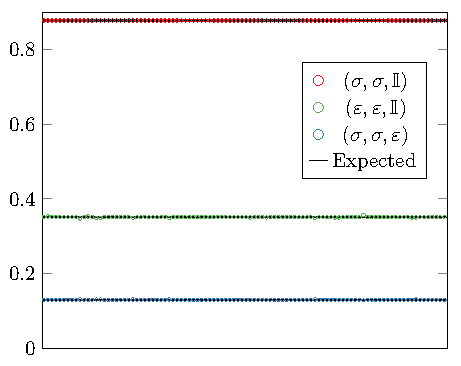
\includegraphics[width=\textwidth]{bootstrap_ising_3.pdf}
\end{minipage}
\vspace{0.75cm}

\begin{minipage}{0.5\linewidth}
\centering
\begin{tabular}{|c|c|}
\multicolumn{2}{c}{$c=-22/5$}\\
\hline 
  $(h_1, h_2, h_3)$ &  $D_{h_1 h_2 h_3}$ \\ 
 \hline
 $(\varphi, \varphi, \mathbb{I})$ &  $\phantom{-}1.51982706 \, (8.9\times 10^{-6})$      \\
 $(\varphi, \varphi, \varphi)$ &    $-6.84471259 \, (8.5\times 10^{-6})$     \\
 \hline
\end{tabular}
\end{minipage}
\begin{minipage}{0.5\linewidth}
 \centering
 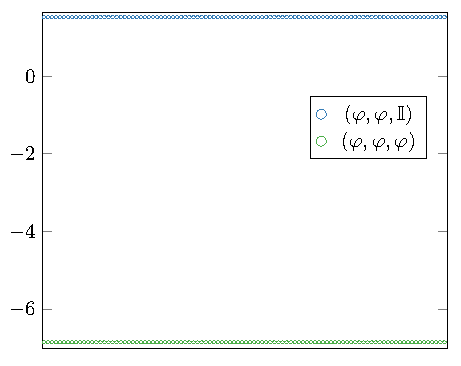
\includegraphics[width=\textwidth]{bootstrap_lee-yang_3.pdf}
\end{minipage}
\vspace{0.75cm}

\begin{minipage}{0.5\linewidth}
\centering
\begin{tabular}{|c|c|}
\multicolumn{2}{c}{$c=-3/5$}\\
\hline 
  $(h_1, h_2, h_3)$ &  $D_{h_1 h_2 h_3}$ \\ 
 \hline
 $(\sigma, \sigma, \mathbb{I})$ &            $\phantom{-}1.11011152\,(4.1\times10^{-4})$        \\
 $(\varepsilon, \varepsilon, \mathbb{I})$ &  $\phantom{-}0.65786020\,(1.0\times10^{-3})$        \\
 $(\psi, \psi, \mathbb{I})$   &              $\phantom{-}0.20732789\,(2.1\times10^{-2})$  \\
 $(\sigma, \sigma, \varepsilon)$ &           $-0.24661111\ (4.1\times 10^{-4})$\\
 $(\varepsilon, \varepsilon, \varepsilon)$ & $-2.33587779\, (2.2\times 10^{-3})$ \\
 $(\sigma, \varepsilon, \psi)$ &             $\phantom{-}0.09693064\,(1.1\times 10^{-2})$\\
 \hline
\end{tabular}
\end{minipage}
\begin{minipage}{0.5\linewidth}
 \centering 
 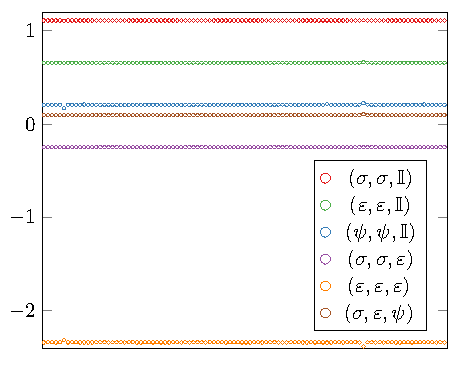
\includegraphics[width=\textwidth]{bootstrap_5-3_3.pdf}
\end{minipage}
\caption{\label{tab_bootstrap_results} Results of the numerical bootstrap for 
the Ising field theory (top), Lee-Yang model (center), and the Gaffnian theory (bottom) 
on a genus two surface ($N=3$). For each minimal model, the table on the left 
collects the mean value obtained for each structure constant after performing the bootstrap
with 100 different sets of random points $\{z_j\}$, fixing $\kappa=0.22$. The conformal block
expansion was truncated at level $\ell=6$. In the brackets we write the coefficient of variation.
In the figures on the right, we plot the values obtained for the structure constants
in each particular set of random points. These are the points employed to calculate the mean and 
standard deviation in the tables on the left. In the Ising theory case, the lines represent the values expected
for the structure constants: $D_{\sigma\sigma\mathbb{I}}\approx 0.877383$, 
$D_{\varepsilon\varepsilon\mathbb{I}}\approx 0.351166$, and $D_{\sigma\sigma\varepsilon}\approx 0.129983$. }
\end{table}


\section{Conclusions}
In this paper we solved numerically the conformal bootstrap to calculate genus two partition functions of rational CFTs, $\mathcal{C}$, with $c<1$. In particular, we focussed on CFTs defined on genus two Riemann surfaces with $\mathbb Z_3$ symmetry, whose partition function can be also rewritten as a twist field four-point function in the orbifold $\mathcal{C}^{\otimes N}/\mathbb Z_N$. Our results extend the approach to higher genus CFTs discussed in~\cite{Cardy, Collier}. In particular we provided a regularization scheme to remove from the combinatorial expansion of the conformal block null vector contributions for $c<1$. We also proposed an algorithm to systematically expand the genus $N-1$ conformal blocks into sphere conformal blocks of central charge $Nc$. The latter are more suitable to implement numerical calculations, since they can represented recursively through Zamolodchikov formula.
Our main results are the exact numerical determinations of the genus two partition functions for the Ising, the Lee-Yang and the Gaffian CFT. The Ising case shows perfect agreement with the free bosonic string calculation in~\cite{Calabrese}.

There are a couple of possibile future directions that are worth to be mentioned. First, it would be useful to investigate whether our formalism can be extended to arbitray values of the genus $g=N-1$. This task involves the determination of the descendent $N$-point function in Eq.~\eqref{N-point} for a rational CFT.  We expect the latter to be analytic in $g$  at least for a free compactified boson, thus allowing to recover the results for the entanglement entropy and negativity discussed in~\cite{Calabrese, Furukawa, Calabrese09, CalabreseNeg, Grava} from a different route.
Also it will be important to understand if a recursive formula for higher genus conformal blocks, such as that put forward in~\cite{Cho}, can be effectively implemented when $c<1$, due to the additional null vector resonances.

\appendix
\section{Recults from Virasoro algebra}\label{app_ward}

Consider a CFT on the Riemann sphere parameterized by $z$.
The Virasoro generators are defined by their action on the fields:
\begin{equation}
\label{vir_ln}
 L_{-n}(z)X^{M}_h(z)=-\oint_{C_{z}}\frac{dz'}{2\pi i}(z'-z)^{n+1}~T(z')~X^{M}_h(z),
\end{equation}
where $C_{z}$ is a closed contour containing $z$ and $T(z)$ is the stress energy tensor. 
From the current-current OPE
\begin{equation}
T(z) T(0)= \frac{c}{z^4}+ \frac{2}{z^2} T(0)+\frac{1}{z}\partial T (0)+\text{regular terms},
\end{equation} 
one obtains the  Virasoro algebra
\begin{equation}
 [L_n(0), L_{m}(0)]X^{M}_h(0) =\left[(n-m) L_{n+m}(0)+\frac{c}{12}n(n^2-1)\delta_{n+m, 0}\right]X^{M}_h(0).
\end{equation}

We want to show now how the descendant fields transforms under a conformal map:
\begin{equation}
t \mapsto z(t)
\end{equation}
To do that, by using the transformation of the stress energy tensor under a conformal map,
\begin{equation}
T(z)\mapsto \left(\frac{d z}{d t}\right)^{-2} T(z(t))-\frac{c}{12}\left\{z(t),t\right\},
\end{equation}
where $\{z(t),t\}$ is the Shwartzian derivative,  in the Eq.(\ref{vir_ln}), one obtains the relation between the modes $L_{n}$ on the $z$ plane and the modes $\mathcal{L}_n(t)$ on the t plane:
\begin{equation}\label{gengen}
\begin{aligned}
 \mathcal{L}_{n}(t)&=\frac{c}{12} \oint_{\mathcal{C}_t}\frac{d t'}{2\pi i}\, (t'-t)^{n+1}\left\{z(t'),t'\right\} +\\
 & +\left(\frac{d z(t)}{d t}\right)^{-n} L_n^{(z(t))}
 +\frac{1-n}{2}\frac{\left.\frac{d^2 z(t)}{d t^2}\right|_{t=t'}}{\left(\frac{d z(t)}{d t}\right)^{n+2}}L_{n+1}^{(z(t))}+\cdots
 \end{aligned}
\end{equation}
We now illustrate an application of Eq.~\eqref{conformal_block_decomposition} to a flat torus. For $N=2$, the three-point function of Eq.~\eqref{orbifold_three-point} 
can be calculated by considering the  one-to-two map (\ref{g_one_covering_map})

which transforms $z=\infty$ into $t_{\infty}=\{0,\infty\}$
in the $t$-plane and has branch points of order two at $z_b=\{0,1\}$.  For the mapping in Eq.~\eqref{g_one_covering_map}, 
we can write down  the expansion of the Virasoro descendents in Eq.~\eqref{Virasoro_transf};
if $n\geq 1$ it reads
\begin{equation}
\label{g1_1}
 \mathcal{L}_{-n}(t_{\infty})=\sum_{m\geq -n} a_{nm} L_{m}(t=t_{\infty})+\frac{c}{32}(n-1), \quad t_{\infty}=\{0,\infty\},
\end{equation}
with
\begin{equation}
\label{g1_2}
 a_{nm}=\frac{1}{4^n}\left[2^{2n+1}-\binom{2n+1}{m+n+1}{}_2F_1(1, m-n, m+n+2, -1)\right].
\end{equation}

Under the conformal map of
Eq.~\eqref{g_one_covering_map}, the Virasoro descendent in Eq.~\eqref{vir_infty}
is then transformed into the linear combination of descendents in the $t$-plane
\begin{equation}\label{Virasoro_transf}
 \mathcal{L}_{-n}(t_{\infty})=-\oint_{C_{t_{\infty}}}\frac{dt}{2\pi i}
 \left(\frac{dz}{dt}\right)^{-1}[z(t)]^{n+1}
 \left[T(t)-\frac{c}{12}\{z(t), t\}\right],
\end{equation}
where $C_{t_{\infty}}$ is a contour encircling the point $t_{\infty}$.
The three-point correlations on the sphere which appear 
in the expansion in Eq.~\eqref{genus_two_conf_block} of the genus two conformal block can be 
computed recursively by employing the following Ward identities~\cite{Teschner},
\begin{multline}
\label{wardvir1}
 \langle L_{-n}X_{h_1}^{M_1}|X_{h_2}^{M_2}(1)|X_{h_3}^{M_3}\rangle=
 \langle X_{h_1}^{M_1}|X_{h_2}^{M_2}(1)|L_n X_{h_3}^{M_3}\rangle \\
 +\sum_{m= 1}^n \binom{n+1}{m+1}\langle X_{h_1}^{M_1}|L_m X_{h_2}^{M_2}(1)|X_{h_3}^{M_3}\rangle,
\end{multline}
\begin{multline}
\label{wardvir2}
 \langle X_{h_1}^{M_1}|L_{-n}X_{h_2}^{M_2}(1)|X_{h_3}^{M_3}\rangle=
 \sum_{m=0}^\infty\binom{n+m-2}{m}
 \left[\langle L_{m+n} X_{h_1}^{M_1}|X_{h_2}^{M_2}(1)|X_{h_3}^{M_3}\rangle \right.\\ +
 \left. (-1)^n\langle X_{h_1}^{M_1}|X_{h_2}^{M_2}(1)|L_{m-1} X_{h_3}^{M_3}\rangle\right],
\end{multline}
and
\begin{equation}
 \langle \phi_{h_1}|\phi_{h_2}(1)|L_{-n}\phi_{h_3}\rangle=
 \langle L_{-n}\phi_{h_3}|\phi_{h_2}(1)|\phi_{h_1}\rangle.
\end{equation}





\section{Zamolodchikov recursion for sphere conformal blocks}\label{app_zamolodchikov}
The sphere conformal block $\mathcal{F}_{Nc, h}(z)$
for central charge $Nc$, internal dimension $h$, and the four
external legs with the same dimension $h_{\sigma_N}$ can be efficiently computed 
using the formula \cite{Zamolodchikov}
\begin{equation}
 \mathcal{F}_{Nc, h}(z)=
 16^{\frac{1-Nc}{24}}q^{h-\frac{Nc-1}{24}}
 [z(1-z)]^{\frac{Nc-1}{24}-2h_{\sigma_N}}
 \vartheta_3(q)^{\frac{Nc-1}{2}-16h_{\sigma_N}}H(Nc, h, h_{\sigma_N}, q),
\end{equation}
where $\vartheta_3(q)$ is the Jacobi theta function and $H(Nc, h, h_{\sigma_N}, q)$
satisfies the recursion relation 
\begin{equation}
 H(Nc, h, h_{\sigma_N}, q)=
 1+\sum_{m, n}\frac{(16q)^{mn}R_{m,n}(Nc, h_{\sigma_N})H(Nc, h_{m,n}+mn, h_{\sigma_N}, q)}
 {h-h_{m,n}(Nc)}.
\end{equation}
The explicit expressions of $h_{m,n}(Nc)$ and $R_{m, n}(Nc, h_{\sigma_N})$
are given by Eqs. (3) and (17) of Ref.~\cite{Zamolodchikov} respectively.  


\acknowledgments
We thank Andrea Cappelli and Sylvain Ribault for discussions.





% The bibliography will probably be heavily edited during typesetting.
% We'll parse it and, using the arxiv number or the journal data, will
% query inspire, trying to verify the data (this will probalby spot
% eventual typos) and retrive the document DOI and eventual errata.
% We however suggest to always provide author, title and journal data:
% in short all the informations that clearly identify a document.

\begin{thebibliography}{99}

\bibitem{Dubrovin} B. A. Dubrovin, A. T. Fomenko, S. P. Novikov, \textit{Modern Geometry---Methods and Applications Part II. The Geometry and Topology of Manifolds}, Springer (1985).

\bibitem{Whittaker} E.T. Whittaker, G. N. Watson, \emph{A Course in Modern Analysis}, Cambridge University Press (1950).

\bibitem{Lunin} O. Lunin, S. D. Mathur, \emph{Correlation functions for $M(N)/S(N)$ orbifolds}, \href{https://doi.org/10.1007/s002200100431}{\emph{Commun. Math. Phys.} {\bf 219} (2001) 399-442}.

\bibitem{Dixon} L. Dixon, D. Friedan, E. Martinec, S. Shenker, \textit{The conformal field theory of orbifolds}, 
\href{https://doi.org/10.1016/0550-3213(87)90676-6}{\emph{Nucl. Phys. B} {\bf 282} (1987) 13-73}.

\bibitem{DiFrancesco} P. Di Francesco, P. Mathieu, D. Senechal, \textit{Conformal field theory}, Springer (1999)

\bibitem{Knizhnik} V. G. Knizhnik, \emph{Analytic fields on Riemannian surfaces. II}, 
\href{https://doi.org/10.1007/BF01225373}{\emph{Commun. Math. Phys.} {\bf 112}, 567-590 (1987)}.

\bibitem{CardyMod} J. Cardy, \emph{Operator content of two-dimensional conformally invariant theories}, 
\href{https://doi.org/10.1016/0550-3213(86)90552-3}{\emph{Nucl. Phys. B} {\bf 270} [FS16] (1986) 186-204}.

\bibitem{Cappelli} A. Cappelli, C. Itzykson, J.-B. Zuber, \emph{Modular invariant partition functions in two dimensions}, 
\href{https://doi.org/10.1016/0550-3213(87)90155-6}{\emph{Nucl. Phys.B} {\bf 280} [FS18], 445 (1987)}.

\bibitem{Cappelli2} A. Cappelli, C. Itzykson, J.-B. Zuber, \emph{The A-D-E classification of minimal and $A_1^{(1)}$ conformal invariant theories}, \href{https://doi.org/10.1007/BF01221394}{\emph{Commun. Math. Phys.} {\bf 113}, 1-26 (1987)}.

\bibitem{Cardy} J. Cardy, A. Maloney, H. Maxfield, \emph{A new handle on three-point coefficients: OPE asymptotics from genus
two modular invariance}, \href{https://doi.org/10.1007/JHEP10(2017)136}{\emph{JHEP} {\bf 10} (2017) 136}.

\bibitem{ZamolodchikovAT} Al. B. Zamolodchikov, \emph{Conformal scalar field on the hyperelliptic curve and critical Ashkin-Teller multipoint correlation functions}, \href{https://doi.org/10.1016/0550-3213(87)90350-6}{\emph{Nucl. Phys. B} {\bf 63} [FS19] (1987) 481-503}.

\bibitem{BPZ} A. Belavin, A. Polyakov, A. B. Zamolodchikov. \emph{Infinite conformal symmetry in two-dimensional quantum field theory},
\href{https://doi.org/10.1016/0550-3213(84)90052-X}{\emph{Nucl. Phys. B}, {\bf 241} (1984) 333-380}.

\bibitem{Friedan} D. Friedan, Z. Qiu, S. Shenker, \emph{Conformal Invariance, Unitarity, and Critical Exponents in Two Dimensions}, \href{https://doi.org/10.1103/PhysRevLett.52.1575}{\emph{Phys. Rev. Lett}. {\bf 52}, 1575 (1984)}.

\bibitem{Collier} M. Cho, S. Collier, X. Yin, \emph{Genus two modular bootstrap}, \href{https://doi.org/10.1007/JHEP04(2019)022}{\emph{JHEP} {\bf 04} (2019) 22}.

\bibitem{Ribault} S. Ribault, \emph{Conformal field theory on the plane}, \href{https://arxiv.org/abs/1406.4290}{\texttt{arXiv:1406.4290 [hep-th]}}.

\bibitem{Zamolodchikov2} Al.  B.  Zamolodchikov, \emph{Conformal  Symmetry  in  Two  Dimensions: An  Explicit  Recurrence Formula for the  Conformal Partial  Wave  Amplitude}, \href{https://doi.org/10.1007/BF01214585}{\emph{Commun. Math. Phys.} {\bf 96},  419-422  (1984)}.

\bibitem{SV} R. Santachiara, J. Viti, \emph{Local logarithmic correlators as limits of Coulomb gas integrals},
\href{https://doi.org/10.1016/j.nuclphysb.2014.02.022}{\emph{Nucl. Phys. B} {\bf 882} (2014) 229-262}.

\bibitem{Javerzat} N. Javerzat, R. Santachiara, O. Foda, \emph{Notes on the solutions of Zamolodchikov-type recursion relations in Virasoro minimal models}, \href{https://doi.org/10.1007/JHEP08(2018)183}{\emph{JHEP} {\bf 08} (2018) 183}.

\bibitem{Alkalaev} K. B. Alkalaev, V. A. Belavin, \emph{Conformal blocks of $\mathcal{W}_N$
minimal models and AGT correspondence}, \href{https://doi.org/10.1007/JHEP07(2014)024}{\emph{JHEP} {\bf 07} (2014) 024}.

\bibitem{SR} S. Ribault, R. Santachiara, \textit{Liouville theory with a central charge less than one}, 
\href{https://doi.org/10.1007/JHEP08(2015)109}{\emph{JHEP} {\bf 08} (2015) 109}.

\bibitem{Zamolodchikov} Al. B. Zamolodchikov, \emph{Conformal symmetry in two-dimensional space: Recursion representation of conformal
block}, \href{https://doi.org/10.1007/BF01022967}{\emph{Theor. Math. Phys.} {\bf 73}, 1088-1093  (1987)}.

\bibitem{Mussardo} G. Mussardo, \emph{Statistical Field Thoery: An Introduction to Exactly Solved Models in Statistical Physics}, Oxford University Press (2020).

\bibitem{Simon} S H. Simon, E. H. Rezayi, N. R. Cooper, I. Berdnikov, \emph{Construction of a paired wave function for spinless electrons at filling fraction $\nu=2/5$}, \href{https://doi.org/10.1103/PhysRevB.75.075317}{\emph{Phys. Rev. B} {\bf 75}, 075317 (2007)}.

\bibitem{Ardonne} E. Ardonne, J. Gukelberger, A. W. W. Ludwig, S. Trebst, M. Troyer, \emph{Microscopic models of interacting Yang-Lee anyons},
\href{https://doi.org/10.1088/1367-2630/13/4/045006}{\emph{New J. Phys.} {\bf 13} (2011) 045006}.

\bibitem{Calabrese} P. Calabrese, J. Cardy, E. Tonni, \emph{Entanglement entropy of two disjoint intervals in conformal field theory II}, \href{https://doi.org/10.1088/1742-5468/2011/01/P01021}{\emph{J. Stat. Mech} P01021 (2011)}.

\bibitem{Rajabpour} M. A. Rajabpour, F. Gliozzi, \emph{Entanglement entropy of two disjoint intervals from fusion algebra of twist fields},
\href{https://doi.org/10.1088/1742-5468/2012/02/P02016}{J. Stat. Mech. (2012) P02016}.

\bibitem{Ruggiero} P. Ruggiero, P. Calabrese, E. Tonni, \emph{Entanglement entropy of two disjoint intervals and the recursion formula
for conformal blocks}, \href{https://doi.org/10.1088/1742-5468/aae5a8}{\emph{J. Stat. Mech.} (2018) 113101}.

\bibitem{Furukawa}  S. Furukawa, V. Pasquier, J. Shiraishi, \emph{Mutual Information and Boson Radius in $c=1$ Critical Systems in One Dimension}, \href{https://doi.org/10.1103/PhysRevLett.102.170602}{\emph{Phys. Rev. Lett.} {\bf 102}, 170602 (2009)}.

\bibitem{Calabrese09} P. Calabrese, J. Cardy, E. Tonni, \emph{Entanglement entropy of two disjoint intervals in conformal field theory},
\href{https://doi.org/10.1088/1742-5468/2009/11/P11001}{J. Stat. Mech (2009) P11001}.

\bibitem{CalabreseNeg} P. Calabrese, J. Cardy, E. Tonni, \emph{Entanglement negativity in extended systems:  A field theoretical approach},
\href{https://doi.org/10.1088/1742-5468/2013/02/P02008}{J. Stat. Mech. (2013) P02008}.

\bibitem{Grava} T. Grava, A. P. Kels, E. Tonni, \emph{Entanglement of two disjoint intervals in CFT and the 2D Coulomb gas in a lattice},
\href{https://arxiv.org/abs/2104.06994}{\texttt{arXiv:2104.06994 [hep-th]}}.

\bibitem{Cho} M. Cho, S. Collier, X. Yin, \emph{Recursive representations of arbitrary Virasoro conformal blocks}, 
\href{https://doi.org/10.1007/JHEP04(2019)018}{\emph{JHEP} {\bf 04} (2019) 018}.

\bibitem{Teschner} J. Teschner, \emph{Liouville theory revisited}, \href{https://doi.org/10.1088/0264-9381/18/23/201}{\emph{Class. Quantum Grav.} {\bf 18} (2001) R153-R222}.

\bibitem{FS} D. Friedan, S. Shenker, \emph{The analytic geometry of two-dimensional conformal field theories}, \href{https://doi.org/10.1016/0550-3213(87)90418-4}{\emph{Nucl. Phys. B} {\bf 281} (1987) 509-545}.

\bibitem{Gaberdiel} M. R. Gaberdiel, C. A. Keller, R. Volpato, \emph{Genus two partition functions of chiral conformal field theories},
\href{https://dx.doi.org/10.4310/CNTP.2010.v4.n2.a2}{\emph{Commun. Num. Theor. Phys.} {\bf 4} (2010) 295-364}.

\bibitem{Headrick} M. Headrick, A. Maloney, E. Perlmutter, I. G. Zadeh, \emph{Renyi Entropies, the Analytic Bootstrap, and 3D Quantum Gravity at Higher Genus}, \href{https://doi.org/10.1007/JHEP07(2015)059}{\emph{JHEP} {\bf 07} (2015) 059}.

\bibitem{Keller} C. A. Keller, G. Mathys, I. G. Zadeh, \emph{Bootstrapping chiral CFTs at genus two},
\href{https://dx.doi.org/10.4310/ATMP.2018.v22.n6.a3}{\emph{Adv. Theor. Math. Phys.} {\bf 22} (2018) 1447-1487}

\bibitem{Dupic} T. Dupic, B. Estienne, Y. Ikhlef, \emph{Entanglement entropies of minimal models from null-vectors}, 
\href{https://scipost.org/10.21468/SciPostPhys.4.6.031}{\emph{SciPost Phys.} {\bf 4}, 031 (2018)}


% Please avoid comments such as "For a review'', "For some examples",
% "and references therein" or move them in the text. In general,
% please leave only references in the bibliography and move all
% accessory text in footnotes.

% Also, please have only one work for each \bibitem.


\end{thebibliography}
\end{document}
